\documentclass[ 12pt, twocolumn]{article}    % two-column because cheat sheets fit like that
\usepackage[utf8]{inputenc}
\usepackage{amsmath}    % allows math to happen
\usepackage{marvosym}
\usepackage{textcomp}
\usepackage{geometry}   % allows you to change the margins and headers/footers, and more
\usepackage{array}
\usepackage{wrapfig}
\usepackage{multirow} 
\usepackage{graphicx}   % allows for inclusion of graphics or several types, i think
\usepackage{float}      % SUPER  IMPORTANT. lets you tell LaTeX where to put your graphics, as opposed to where it feels
\usepackage{wrapfig}    % Lets text wrap around figures, more relevant for reports really
\usepackage{caption}
\usepackage{amssymb}    
\usepackage{ulem}       % allows strikethrough and some
\usepackage[table]{xcolor}  % enhances tables by allowing colors to happen. notably, as background/fill colors

\usepackage{booktabs}% http://ctan.org/pkg/booktabs
\newcommand{\tabitem}{~~\llap{\textbullet}~~}   % for making lists in tables
\usepackage{multicol}
\usepackage{bondgraph}  % allows bond graphs
\usepackage{caption}    % lots of control of captions and caption geometries
\usepackage{comment}

\geometry{margin=.5in}      % this allows for a lot to fit on the page

\begin{document}
\footnotesize                      % small because, it's a cheat sheet after all, why not cram it
\captionsetup{aboveskip=-100pt}
\captionsetup{belowskip=-100pt}

\section*{System Dynamics}




\begin{figure}[h]
    \centering
    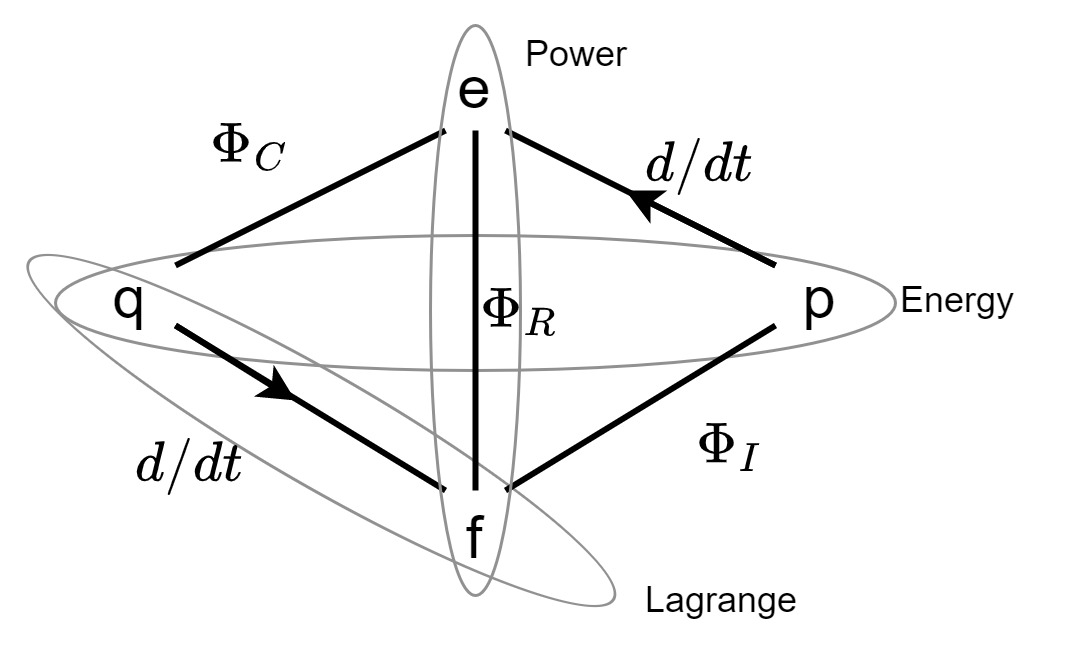
\includegraphics[width =0.4\textwidth]{TetrahedronOfState.jpg}
\end{figure}

%%
\subsection*{Element (and Field) Types}
\noindent
\underline{Reactance(s)}

\begin{itemize}
    \item Efforts and flows
    \item \emph{Cannot} store energy. Power conservative or power dissipative 
    \item Hydraulic: \(P_{12} = \Phi_RQ = \alpha Q|Q|\) 
\end{itemize}

\begin{center}
    Resistance form \hspace{30pt} Conductance form\\
    \begin{footnotesize}
        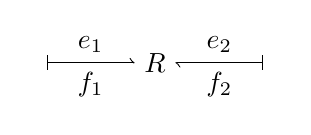
\begin{tikzpicture}[node distance=1.5cm]
            \bgComponentNoBond{empty1}{}
            \bgComponentWithBondLabel{}{R1}{\(R\)}{right of=}{empty1}{inbondf}{}{\(e_1\)}{\(f_1\)}
            \bgComponentWithBondLabel{}{empty2}{}{right of=}{R1}{outbondf}{}{\(e_2\)}{\(f_2\)}
        \end{tikzpicture}
        \hspace{10pt} 
        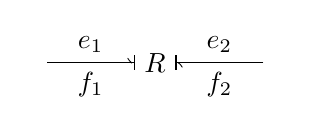
\begin{tikzpicture}[node distance=1.5cm]
            \bgComponentNoBond{empty1}{}
            \bgComponentWithBondLabel{}{R1}{\(R\)}{right of=}{empty1}{inbonde}{}{\(e_1\)}{\(f_1\)}
            \bgComponentWithBondLabel{}{empty2}{}{right of=}{R1}{outbonde}{}{\(e_2\)}{\(f_2\)}
        \end{tikzpicture}
    \end{footnotesize}
\end{center}
%
\begin{equation*}
    \textbf{e} = \textbf{\(\Phi\)}_R (\textbf{f}) \hspace{70pt} \textbf{f} = \textbf{\(\Phi\)}_R^{-1} (\textbf{e})
\end{equation*}

In conductance form:
\begin{equation*}
    f_2 = \frac{e_1-e_2}{R} \hspace{30pt} f_1 = \frac{e_2-e_1}{R}
\end{equation*}


%%
\noindent
\underline{Capacitance(s)}
\begin{itemize}
    \item Efforts and displacements
    \item \(e = \Phi_C(q)\)
    \item Hydraulic: \(P = \rho gh = \rho g\frac{V}{A} = \frac{1}{C_f} V\)
\end{itemize}
\begin{center}
    \begin{footnotesize}
	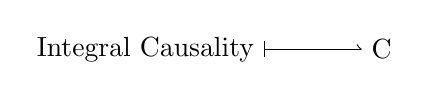
\begin{tikzpicture}[node distance=3cm]
		\bgComponentNoBond{Se1}{Integral Causality}
		\bgComponent{}{C1}{C}{right of=}{Se1}{inbondf}
	\end{tikzpicture}
	\end{footnotesize}
\end{center}
%
\begin{center}
    \begin{footnotesize}
    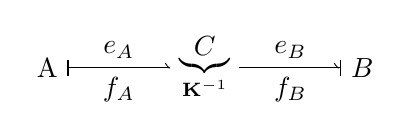
\begin{tikzpicture}[node distance=2cm]
        \bgComponentNoBond{A1}{A }
        \bgComponentWithBondLabel{}{C1}{\(\underbrace{C}_{\textbf{K}^{-1}}\)}{right of=}{A1}{inbondf}{}{\(e_A\)}{\(f_A\)}
        \bgComponentWithBondLabel{}{B1}{\(B\)}{right of=}{C1}{inbonde}{}{\(e_B\)}{\(f_B\)}
    \end{tikzpicture}
    \end{footnotesize}        
\end{center}
%
\begin{equation*}
    \begin{bmatrix}
        e_A\\ e_B
    \end{bmatrix} 
    = 
    \textbf{K} 
    \begin{bmatrix}
        q_A\\ q_B
    \end{bmatrix} 
\end{equation*}
\begin{equation*}
    E(\textbf{q}) = \int_0^\textbf{q} \Phi_C(\textbf{q})d\textbf{q} \hspace{30pt}  \frac{\partial{e_i}}{\partial{q_j}} =  \frac{\partial{e_j}}{\partial{q_i}}
\end{equation*}


%%
\noindent
\underline{Inertance(s)}
\begin{itemize}
    \item Flows and momenta
    \item \(e = \int \Phi_I (p) dp\)  or  \(f = p/I\)
    \item Hydraulic: \(p_{p_3} = \int ( P_1 - P_2) dt \Longrightarrow \Dot{p_{p_3}} = P_1 - P_2\)
    \begin{itemize}
        \item \(Q = \frac{A}{\rho L } p_p = \frac{1}{I_f} p_p \Longrightarrow\) Long thin pipes 
        \item Pressure drop = \(d/dt\)(hydraulic momentum)
    \end{itemize}
    \item Electrical: \(p_L = Li\) (flux linkage)
\end{itemize}
\begin{center}
    \begin{footnotesize}
	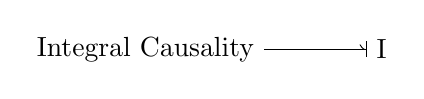
\begin{tikzpicture}[node distance=3cm]
		\bgComponentNoBond{Se1}{Integral Causality}
		\bgComponent{}{I1}{I}{right of=}{Se1}{inbonde}
	\end{tikzpicture}
	\end{footnotesize}
\end{center}
%
\begin{center}
    \begin{footnotesize}
        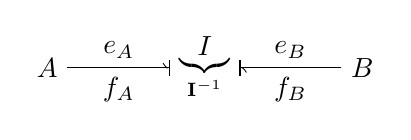
\begin{tikzpicture}[node distance=2cm]
            \bgComponentNoBond{A1}{\(A\)}
            \bgComponentWithBondLabel{}{I1}{\(\underbrace{I}_{\textbf{I}^{-1}}\)}{right of=}{A1}{inbonde}{}{\(e_A\)}{\(f_A\)}
            \bgComponentWithBondLabel{}{B1}{\(B\)}{right of=}{I1}{outbonde}{}{\(e_B\)}{\(f_B\)}
        \end{tikzpicture}
    \end{footnotesize}
\end{center}
%
\begin{equation*}
    \begin{bmatrix}
        f_A \\ f_B
    \end{bmatrix}
    = \textbf{I}^{-1} 
    \begin{bmatrix}
        p_A \\ p_B
    \end{bmatrix}
\end{equation*}
\begin{equation*}
    E(\textbf{p}) = \int_0^\textbf{p} \textbf{\(\Phi\)}_I(\textbf{p})d\textbf{p} \hspace{30pt}  \frac{\partial{f_i}}{\partial{p_j}} =  \frac{\partial{f_j}}{\partial{p_i}}
\end{equation*}

%%
\noindent
\underline{IC-Fields}
\begin{itemize}
    \item Flows and momenta, efforts and displacements 
    \item Two forms of energy storage 
\end{itemize}
\begin{equation*}
    \begin{bmatrix}
        f_1\\ \vdots \\ f_j \\
        e_{j+1} \\ \vdots \\ e_n
    \end{bmatrix}
    = \textbf{IC} 
    \begin{bmatrix}
        p_1 \\ \vdots\\ p_j\\
        q_{j+1} \\ \vdots \\ q_n
    \end{bmatrix} \hspace{30pt}  \frac{\partial{f_i}}{\partial{q_k}} =  \frac{\partial{e_k}}{\partial{p_i}}
\end{equation*}
\begin{equation*}
    E = \underbrace{ \sum_{i=0}^j \int_0^{p_i} f_idp_i}_{\text{I portion}} + \underbrace{\sum_{k=j+1}^n \int_0^{q_k} e_kdq_k}_{\text{C portion}}
\end{equation*}

%%
\noindent
\underline{Sources/Sinks}
\begin{center}
    \begin{footnotesize}
	\begin{tikzpicture}[node distance=1.5cm]
		\bgComponentNoBond{Se1}{\(S_e\)}
		\bgComponent{}{C1}{}{right of=}{Se1}{inbonde}
    \end{tikzpicture}
    \hspace{40pt}
    \begin{tikzpicture}[node distance=1.5cm]
        \bgComponentNoBond{Sf1}{\(S_f\)}
		\bgComponent{}{C1}{}{right of=}{Sf1}{inbondf}
	\end{tikzpicture}	
	\end{footnotesize}
\end{center}

%%
\noindent
\underline{Transducers}
\begin{center}
        \begin{footnotesize}
    \begin{tikzpicture}[node distance=1.5cm]
        \bgComponentNoBond{empty1}{}
        \bgComponent{}{GY1}{GY}{right of=}{empty1}{inbonde}
        \bgComponent{}{empty2}{}{right of=}{GY1}{inbondf}
    \end{tikzpicture}
    \hspace{10pt} OR \hspace{10pt}
    \begin{tikzpicture}[node distance=1.5cm]
        \bgComponentNoBond{empty1}{}
        \bgComponent{}{GY1}{GY}{right of=}{empty1}{inbondf}
        \bgComponent{}{empty2}{}{right of=}{GY1}{inbonde}
    \end{tikzpicture}
    \end{footnotesize}
\end{center}
%
\begin{center}
    \begin{footnotesize}
    \begin{tikzpicture}[node distance=1.5cm]
        \bgComponentNoBond{empty1}{}
        \bgComponent{}{TF1}{TF}{right of=}{empty1}{inbonde}
        \bgComponent{}{empty2}{}{right of=}{TF1}{inbonde}
    \end{tikzpicture}
    \hspace{10pt} OR \hspace{10pt}
    \begin{tikzpicture}[node distance=1.5cm]
        \bgComponentNoBond{empty1}{}
        \bgComponent{}{TF1}{TF}{right of=}{empty1}{inbondf}
        \bgComponent{}{empty2}{}{right of=}{TF1}{inbondf}
    \end{tikzpicture}
    \end{footnotesize}
\end{center}

%%
\noindent
\underline{Multi-port Transformers}
\vspace{10pt}
\newline
An example of a simplified system, where \(\textbf{M}\) comes from the original Bond Graph to satisfy the following two equations:
\begin{equation*}
    \begin{bmatrix}
        f_C\\ f_D
    \end{bmatrix} 
    = \textbf{M}
    \begin{bmatrix}
        f_A\\ f_B
    \end{bmatrix} \hspace{50pt} 
    \begin{bmatrix}
        e_A\\ e_B 
    \end{bmatrix}
    = \textbf{M}^T 
    \begin{bmatrix}
        e_C\\ e_D
    \end{bmatrix}
\end{equation*}
%
\begin{center}
        \begin{footnotesize}
        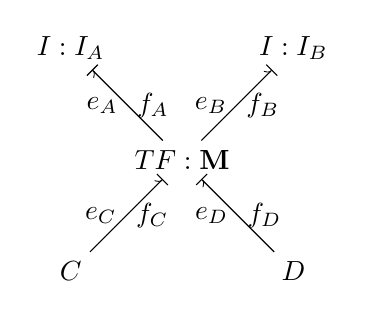
\begin{tikzpicture}[node distance=2cm]
            \bgComponentNoBond{I1}{\(I:I_A\)}
            \bgComponentWithBondLabel{}{TF1}{\(TF:\textbf{M}\)}{below right of=}{I1}{outbonde}{}{\(e_A\)}{\(f_A\)}
            \bgComponentWithBondLabel{}{I2}{\(I:I_B\)}{above right of=}{TF1}{inbonde}{}{\(e_B\)}{\(f_B\)}
            \bgComponentWithBondLabel{}{C}{\(C\)}{below left of=}{TF1}{outbonde}{}{\(e_C\)}{\(f_C\)}
            \bgComponentWithBondLabel{}{D}{\(D\)}{below right of=}{TF1}{outbonde}{}{\(e_D\)}{\(f_D\)}
        \end{tikzpicture}
    \end{footnotesize}
\end{center}



%%
\newpage
\subsection*{Magnetic Domain}
\begin{figure}[t]
    \centering
    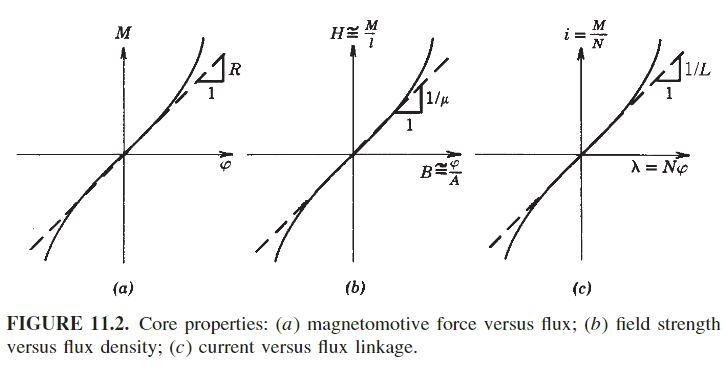
\includegraphics[width=0.49\textwidth]{karnopp_magnetic_properties_plots.jpg}
\end{figure}
\begin{equation*}
    \lambda =N\psi \hspace{30pt} \Dot{\lambda} =N\Dot{\psi} \hspace{30pt} M=Ni
\end{equation*}
\begin{center}
        \begin{footnotesize}
        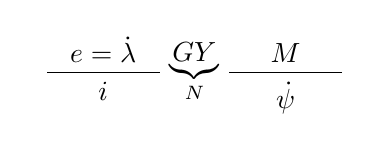
\begin{tikzpicture} [node distance=2cm]
            \bgComponentNoBond{empty1}{}
            \bgComponentWithBondLabel{}{GY1}{\(\underbrace{GY}_{N}\)}{right of=}{empty1}{}{}{\(e=\Dot{\lambda}\)}{\(i\)}
            \bgComponentWithBondLabel{}{empty2}{}{right of=}{GY1}{}{}{\(M\)}{\(\Dot{\psi}\)}
        \end{tikzpicture}
    \end{footnotesize}
\end{center}
\begin{equation*}
    \text{const. law of iron core:  } M = Re\psi = \frac{L}{\mu A} \psi
\end{equation*}
\begin{equation*}
    \text{OR} \hspace{20pt} H = \frac{1}{\mu} B \hspace{30pt} M = \frac{L}{\mu A} \psi
\end{equation*}





Electrical inductances are magnetic capacitances!
\begin{center}
        \begin{footnotesize}
        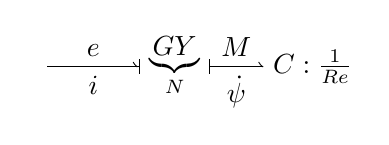
\begin{tikzpicture} [node distance=1.75cm]
            \bgComponentNoBond{empty1}{}
            \bgComponentWithBondLabel{}{GY1}{\(\underbrace{GY}_N\)}{right of=}{empty1}{inbonde}{}{\(e\)}{\(i\)}
            \bgComponentWithBondLabel{}{C1}{\(C:\frac{1}{Re}\)}{right of=}{GY1}{inbondf}{}{\(M\)}{\(\Dot{\psi}\)}
        \end{tikzpicture}
        OR
        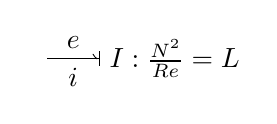
\begin{tikzpicture}[node distance=1.75cm]
            \bgComponentNoBond{empty2}{}
            \bgComponentWithBondLabel{}{I1}{\(I:\frac{N^2}{Re}=L\)}{right of=}{empty2}{inbonde}{}{\(e\)}{\(i\)}
        \end{tikzpicture}
    \end{footnotesize}
\end{center}
\begin{figure}[!h]
    \centering
    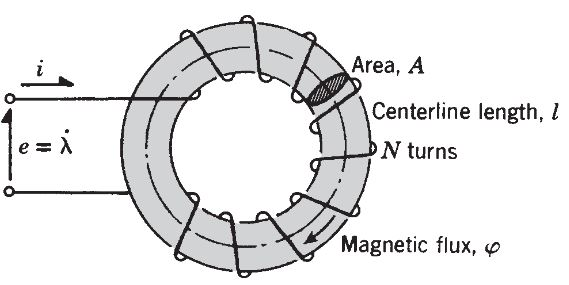
\includegraphics[width =0.35\textwidth]{toroidalCoilSchematic.png}
\end{figure}




%
\noindent
\underline{Example}: Magnetic circuit and Bond Graph:
\begin{figure}[h]
    \centering
    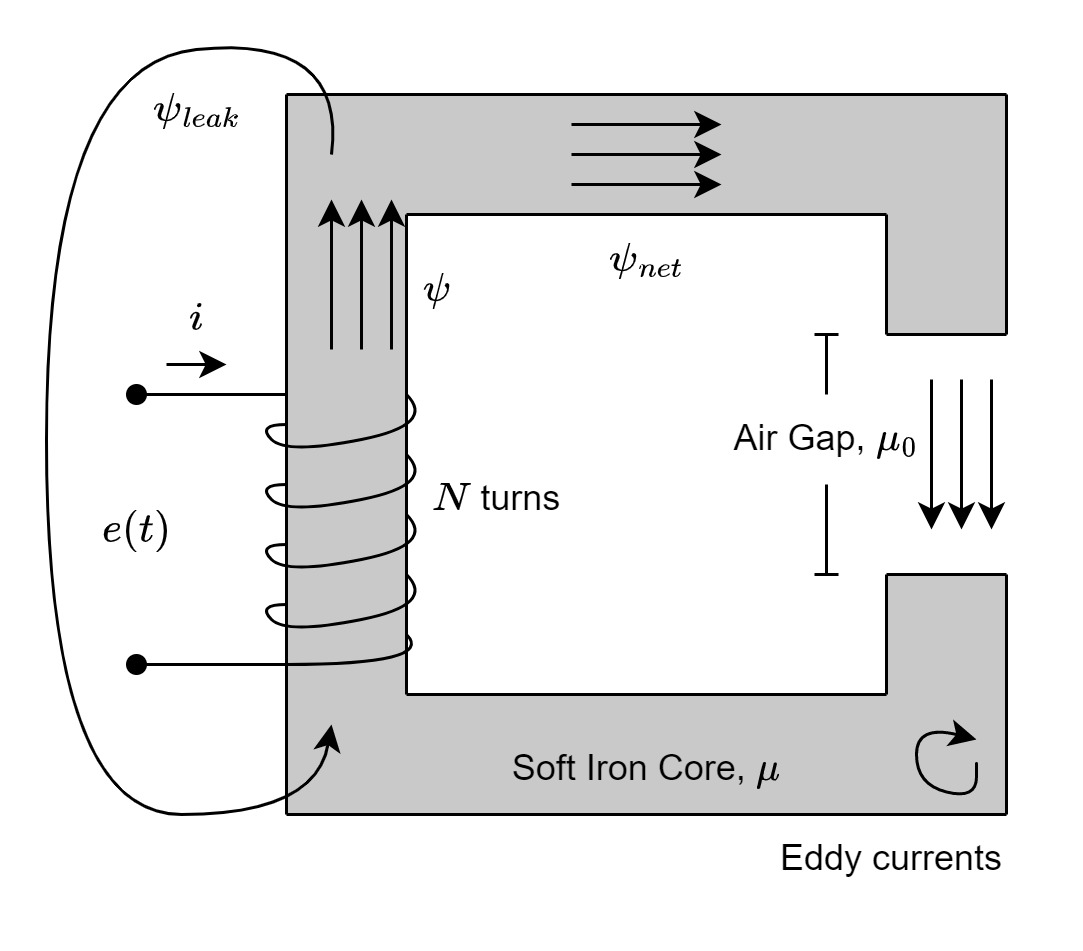
\includegraphics[width=0.30\textwidth]{magneticCircuit.jpg}    
\end{figure}
\begin{center}
       \begin{footnotesize}
        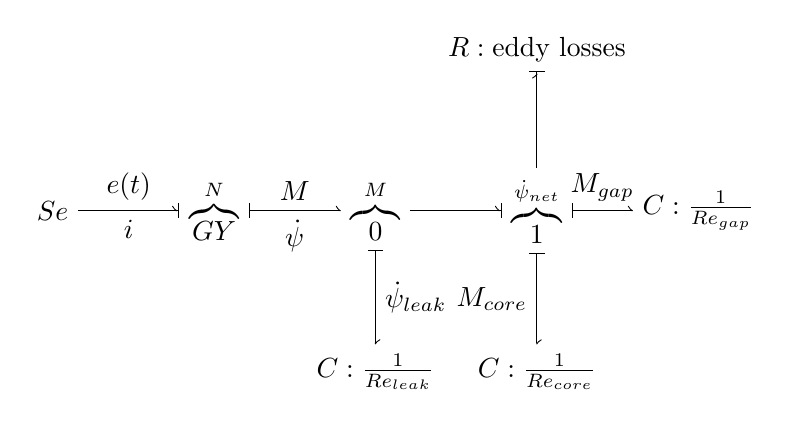
\begin{tikzpicture} [node distance=2.05cm]
            \bgComponentNoBond{Se1}{\(Se\)}
            \bgComponentWithBondLabel{}{GY1}{\(\overbrace{GY}^N\)}{right of=}{Se1}{inbonde}{}{\(e(t)\)}{\(i\)}
            \bgComponentWithBondLabel{}{J01}{\(\overbrace{0}^M\)}{right of=}{GY1}{inbondf}{}{\(M\)}{\(\Dot{\psi}\)}
            \bgComponentWithBondLabel{}{Cleak}{\(C:\frac{1}{Re_{leak}}\)}{below of=}{J01}{inbondf}{}{}{\(\Dot{\psi}_{leak}\)}
            \bgComponentWithBondLabel{}{J11}{\(\overbrace{1}^{\Dot{\psi}_{net}}\)}{right of=}{J01}{inbonde}{}{}{}
            \bgComponentWithBondLabel{}{Ccore}{\(C:\frac{1}{Re_{core}}\)}{below of=}{J11}{inbondf}{}{\(M_{core}\)}{}
            \bgComponentWithBondLabel{}{Cgap}{\(C:\frac{1}{Re_{gap}}\)}{right of=}{J11}{inbondf}{}{\(M_{gap}\)}{}
            \bgComponentWithBondLabel{}{Reddy}{\(R:\text{eddy losses}\)}{above of=}{J11}{inbonde}{}{}{}
        \end{tikzpicture}
    \end{footnotesize}
\end{center}

\noindent
\underline{Permanent Magnets}
\begin{equation*}
    M = M_c-M_0
\end{equation*}
\begin{center}
        \begin{footnotesize}
        \begin{tikzpicture}[node distance=2cm]
            \bgComponentNoBond{Se1}{\(Se\)}
            \bgComponentWithBondLabel{}{J1}{\(\overbrace{1}^{\Dot{\psi}}\)}{right of=}{Se1}{inbond}{}{\(M_0\)}{}
            \bgComponentWithBondLabel{}{C}{\(C:\frac{1}{Re_{PM}}\)}{below of=}{J1}{inbond}{}{\(M_c\)}{}
            \bgComponentWithBondLabel{}{rest}{}{right of=}{J1}{outbond}{}{\(M\)}{}
        \end{tikzpicture}
    \end{footnotesize}
\end{center}
\noindent
\underline{Magnetic Forces}
\begin{enumerate}
    \item Lorentz Force
        \begin{itemize}
            \item  DC motors, voice-coils, etc.
            \item \emph{Cannot} store energy
        \end{itemize}
        \begin{center}
            \begin{footnotesize}
                    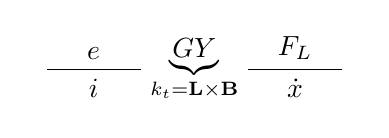
\begin{tikzpicture}[node distance=2cm]
                        \bgComponentNoBond{empty1}{}                    \bgComponentWithBondLabel{}{GY1}{\(\underbrace{GY}_{k_t = \textbf{L} \times \textbf{B} }\)}{right of=}{empty1}{}{}{\(e\)}{\(i\)}
                        \bgComponentWithBondLabel{}{empty2}{}{right of=}{GY1}{}{}{\(F_L\)}{\(\Dot{x}\)}
                    \end{tikzpicture}
                \end{footnotesize}
        \end{center}
   \item Variable reluctance forces
        \begin{equation*}
            e = e(x,\psi) \hspace{20pt} \Longrightarrow \hspace{20pt} \text{C-field}
        \end{equation*}
        \begin{center}
            \begin{footnotesize}
                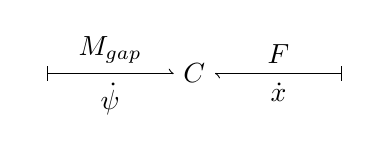
\begin{tikzpicture} [node distance=2cm]
                    \bgComponentNoBond{empty1}{}                    \bgComponentWithBondLabel{}{C1}{\(C\)}{right of=}{empty1}{inbondf}{}{\(M_{gap}\)}{\(\Dot{\psi}\)}
                    \bgComponentWithBondLabel{}{empty2}{}{right of=}{C1}{outbondf}{}{\(F\)}{\(\Dot{x}\)}
                \end{tikzpicture}
            \end{footnotesize}
        \end{center}
        \noindent
        with: \(M=M(x,\psi)\) and \(F=F(x,\psi)\)
\end{enumerate}



%%
\subsection*{Thermodynamic Domain}
\begin{equation*}
    \frac{du}{dt}  = T\Dot{s}-P\dot{v}
\end{equation*}
\begin{equation*}
    PV =mRT \rightarrow Pv = RT \hspace{30pt}  \frac{\partial{T}}{\partial{v}} = \frac{\partial^2u}{\partial v \partial s} =  \frac{\partial{
    (-P)}}{\partial{s}}
\end{equation*}
\begin{equation*}
    \dot{E} =h_{up}\dot{m}_{up} = c_PT_{up}\dot{m}_{up} \hspace{30pt} \dot{m} =\frac{P_{in}-P_{out}}{R}
\end{equation*}
\begin{equation*}
    T =\frac{E}{mc_V}\hspace{30pt} P = \frac{mRT}{V}
\end{equation*}
\begin{center}
    \begin{footnotesize}
        \begin{tikzpicture} [node distance=2cm]
            \bgComponentNoBond{empty1}{}
            \bgComponentWithBondLabel{}{C1}{\(C\)}{right of=}{empty1}{inbond}{}{\(T\)}{\(\Dot{S}\)}
            \bgComponentWithBondLabel{}{empty2}{}{right of=}{C1}{inbond}{}{\(P\)}{\(\Dot{V}\)}
        \end{tikzpicture}
    \end{footnotesize}
\end{center}

\begin{equation*}
    \underbrace{T = T_0 e ^{S/mC_V}\left(\frac{v}{v_0}\right)^{-R/C_V}}_{\text{integral thermal}} \hspace{16pt} \underbrace{S=c_Vln\left(\frac{T}{T_0}\right) +Rln\left(\frac{v}{v_0}\right)}_{\text{derivative thermal}}
\end{equation*}
\begin{equation*}
    \underbrace{P=P_0 e^{S/mc_V}\left(\frac{v}{v_0}\right)^{-c_P/c_V}}_{\text{integral hydraulic}}
\end{equation*}
%
\underline{Special cases}:
\begin{center}
    \begin{footnotesize}
        \begin{tikzpicture} [node distance=2cm]
            \bgComponentNoBond{empty1}{}
            \bgComponentWithBondLabel{}{C1}{\(C\)}{right of=}{empty1}{inbondf}{}{\(T\)}{\(\Dot{S}\)}
            \bgComponentWithBondLabel{}{empty2}{}{right of=}{C1}{inbondf}{}{\(P\)}{\(\Dot{V}\)}
        \end{tikzpicture} \(\overbrace{\dot{h} = \dot{u} + P\dot{v}=T\dot{s}}^{\text{const. pressure, state: \(s\)}} \)
    \end{footnotesize}
\end{center}
\begin{center}
    \begin{footnotesize}
        \begin{tikzpicture} [node distance=2cm]
            \bgComponentNoBond{empty1}{}
            \bgComponentWithBondLabel{}{C1}{\(C\)}{right of=}{empty1}{inbonde}{}{\(T\)}{\(\Dot{S}\)}
            \bgComponentWithBondLabel{}{empty2}{}{right of=}{C1}{inbonde}{}{\(P\)}{\(\Dot{V}\)}
        \end{tikzpicture} \(\overbrace{\dot{f} = \dot{u} - T\dot{s}=-P\dot{v}}^{\text{const. temp, state: \(v\)}} \)
    \end{footnotesize}
\end{center}
\begin{center}
    \begin{footnotesize}
        \begin{tikzpicture} [node distance=2cm]
            \bgComponentNoBond{empty1}{}
            \bgComponentWithBondLabel{}{C1}{\(C\)}{right of=}{empty1}{inbonde}{}{\(T\)}{\(\Dot{S}\)}
            \bgComponentWithBondLabel{}{empty2}{}{right of=}{C1}{inbondf}{}{\(P\)}{\(\Dot{V}\)}
        \end{tikzpicture} \(\overbrace{\dot{\phi} =\dot{u} +P\dot{v} - T\dot{s}=0}^{\text{const. temp \& press, no states} }\)
    \end{footnotesize}
\end{center}
\begin{center}
    \begin{footnotesize}
        \begin{tikzpicture} [node distance=2cm]
            \bgComponentNoBond{empty1}{}
            \bgComponentWithBondLabel{}{C1}{\(C\)}{right of=}{empty1}{inbondf}{}{\(T\)}{\(\Dot{S}\)}
        \end{tikzpicture} \(\overbrace{T = T_0 e^{S/mc_V} }^{\text{isometric (thermal C), } \dot{V}=0}\)
    \end{footnotesize}
\end{center}
\begin{center}
    \begin{footnotesize}
        \begin{tikzpicture} [node distance=2cm]
        \bgComponentNoBond{C1}{\(C\)}
        \bgComponentWithBondLabel{}{empty1}{}{right of=}{C1}{inbonde}{}{\(P\)}{\(\dot{V}\)}
        \end{tikzpicture} \(\overbrace{P=P_0\left(\frac{v}{v_0}\right)^{-c_P/c_V}}^{\text{isentropic (pneumatic C), }\dot{S}=0 }\)
    \end{footnotesize}
\end{center}
    
\noindent
\underline{Heat Transfer}:
\begin{equation*}
\dot{S}_2 - \dot{S}_1 = \frac{H(T_1-T_2)^2}{T_1 T_2} \geq 0
\end{equation*}
\begin{equation*}
\dot{S}_1 =\frac{H(T_1-T_2)}{T_1} \hspace{30pt} \dot{S}_2 = \frac{H(T_1-T_2)}{T_2}
\end{equation*}
\begin{center}
    \begin{footnotesize}
        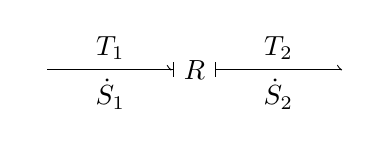
\begin{tikzpicture} [node distance=2cm]
            \bgComponentNoBond{empty1}{}
            \bgComponentWithBondLabel{}{R1}{\(R\)}{right of=}{empty1}{inbonde}{}{\(T_1\)}{\(\dot{S}_1\)}
            \bgComponentWithBondLabel{}{empty2}{}{right of=}{R1}{inbondf}{}{\(T_2\)}{\(\dot{S}_2\)}
        \end{tikzpicture}
    \end{footnotesize}
\end{center}
\begin{itemize}
    \item Conductive causality \(\because \dot{S}_2-\dot{S}_1\geq0\)
    \item All electrical and mechanical R's are actually R-fields with the thermal domain. Causality on the thermal side is enforced, the other is not.
\end{itemize}
\begin{equation*}
    \text{Electro-Thermal} \hspace{50pt} \text{Frictional Heating}
\end{equation*}
\begin{center}
    \begin{footnotesize}
        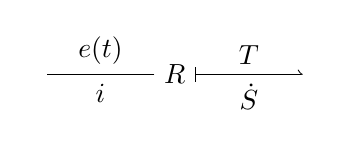
\begin{tikzpicture} [node distance=1.75cm]
            \bgComponentNoBond{empty1}{}
            \bgComponentWithBondLabel{}{R1}{\(R\)}{right of=}{empty1}{}{}{\(e(t)\)}{\(i\)}
            \bgComponentWithBondLabel{}{empty2}{}{right of=}{R1}{inbondf}{}{\(T\)}{\(\dot{S}\)}
        \end{tikzpicture} 
        \hspace{10pt}
        \begin{tikzpicture} [node distance=1.75cm]
            \bgComponentNoBond{empty1}{}
            \bgComponentWithBondLabel{}{R1}{\(R\)}{right of=}{empty1}{inbond}{}{\(F\)}{\(\dot{x}\)}
            \bgComponentWithBondLabel{}{empty2}{}{right of=}{R1}{inbondf}{}{\(T\)}{\(\dot{S}\)}
        \end{tikzpicture}
    \end{footnotesize}
\end{center}


    
%%
\subsection*{Reciprocity and Energy}
\noindent
\underline{Example}:\\
\noindent
A C-field with half constitutive law \(e_1 = e_1(q_1,q_2)\).The energy stored within a C-field is the following:
\begin{equation*}
    E = \int e_1 dq_1 + \int e_2 dq_2
\end{equation*}
\begin{figure}[h]
    \centering
    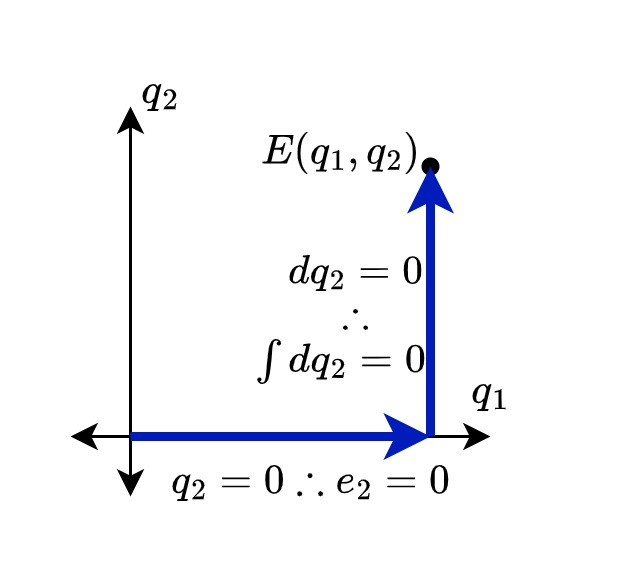
\includegraphics[width=0.3\textwidth]{StateSpaceIntegration.jpg}
\end{figure}
\noindent
Integrating cleverly in state space gives the total energy. Taking a derivative gets the other half of the constitutive law:
\begin{equation*}
     \frac{\partial{E}}{\partial{q_2}} = e_2(q_1,q_2)
\end{equation*}

%%
\subsection*{Linearization}
An example C-field has constitutive law \(V_c = V_c(q,x)\), with nominal values \(V_0\), \(x_0\), \(q_0\). A Taylor-series linearization then yields:
\begin{equation*}
    V_c \approx V_0 +  \left.\frac{\partial{V_c}}{\partial{q}}\right|_{x_0,q_0} \hspace{-20pt} \Delta q + \left. \frac{\partial{V_c}}{\partial{x}} \right|_{x_0,q_0} \hspace{-20pt} \Delta x
\end{equation*}
\noindent
Now, the states are \(\Delta q\) and \(\Delta x\)








% \begin{comment}
%         \begin{figure}[h]
%             \centering
%             \begin{footnotesize}
%                 \begin{tikzpicture} [node distance=2cm]
                    
%                 \end{tikzpicture}
%             \end{footnotesize}
%         \end{figure}
% \end{comment}



% \section*{Causality Procedure}
\begin{figure*}[h]
    \centering
    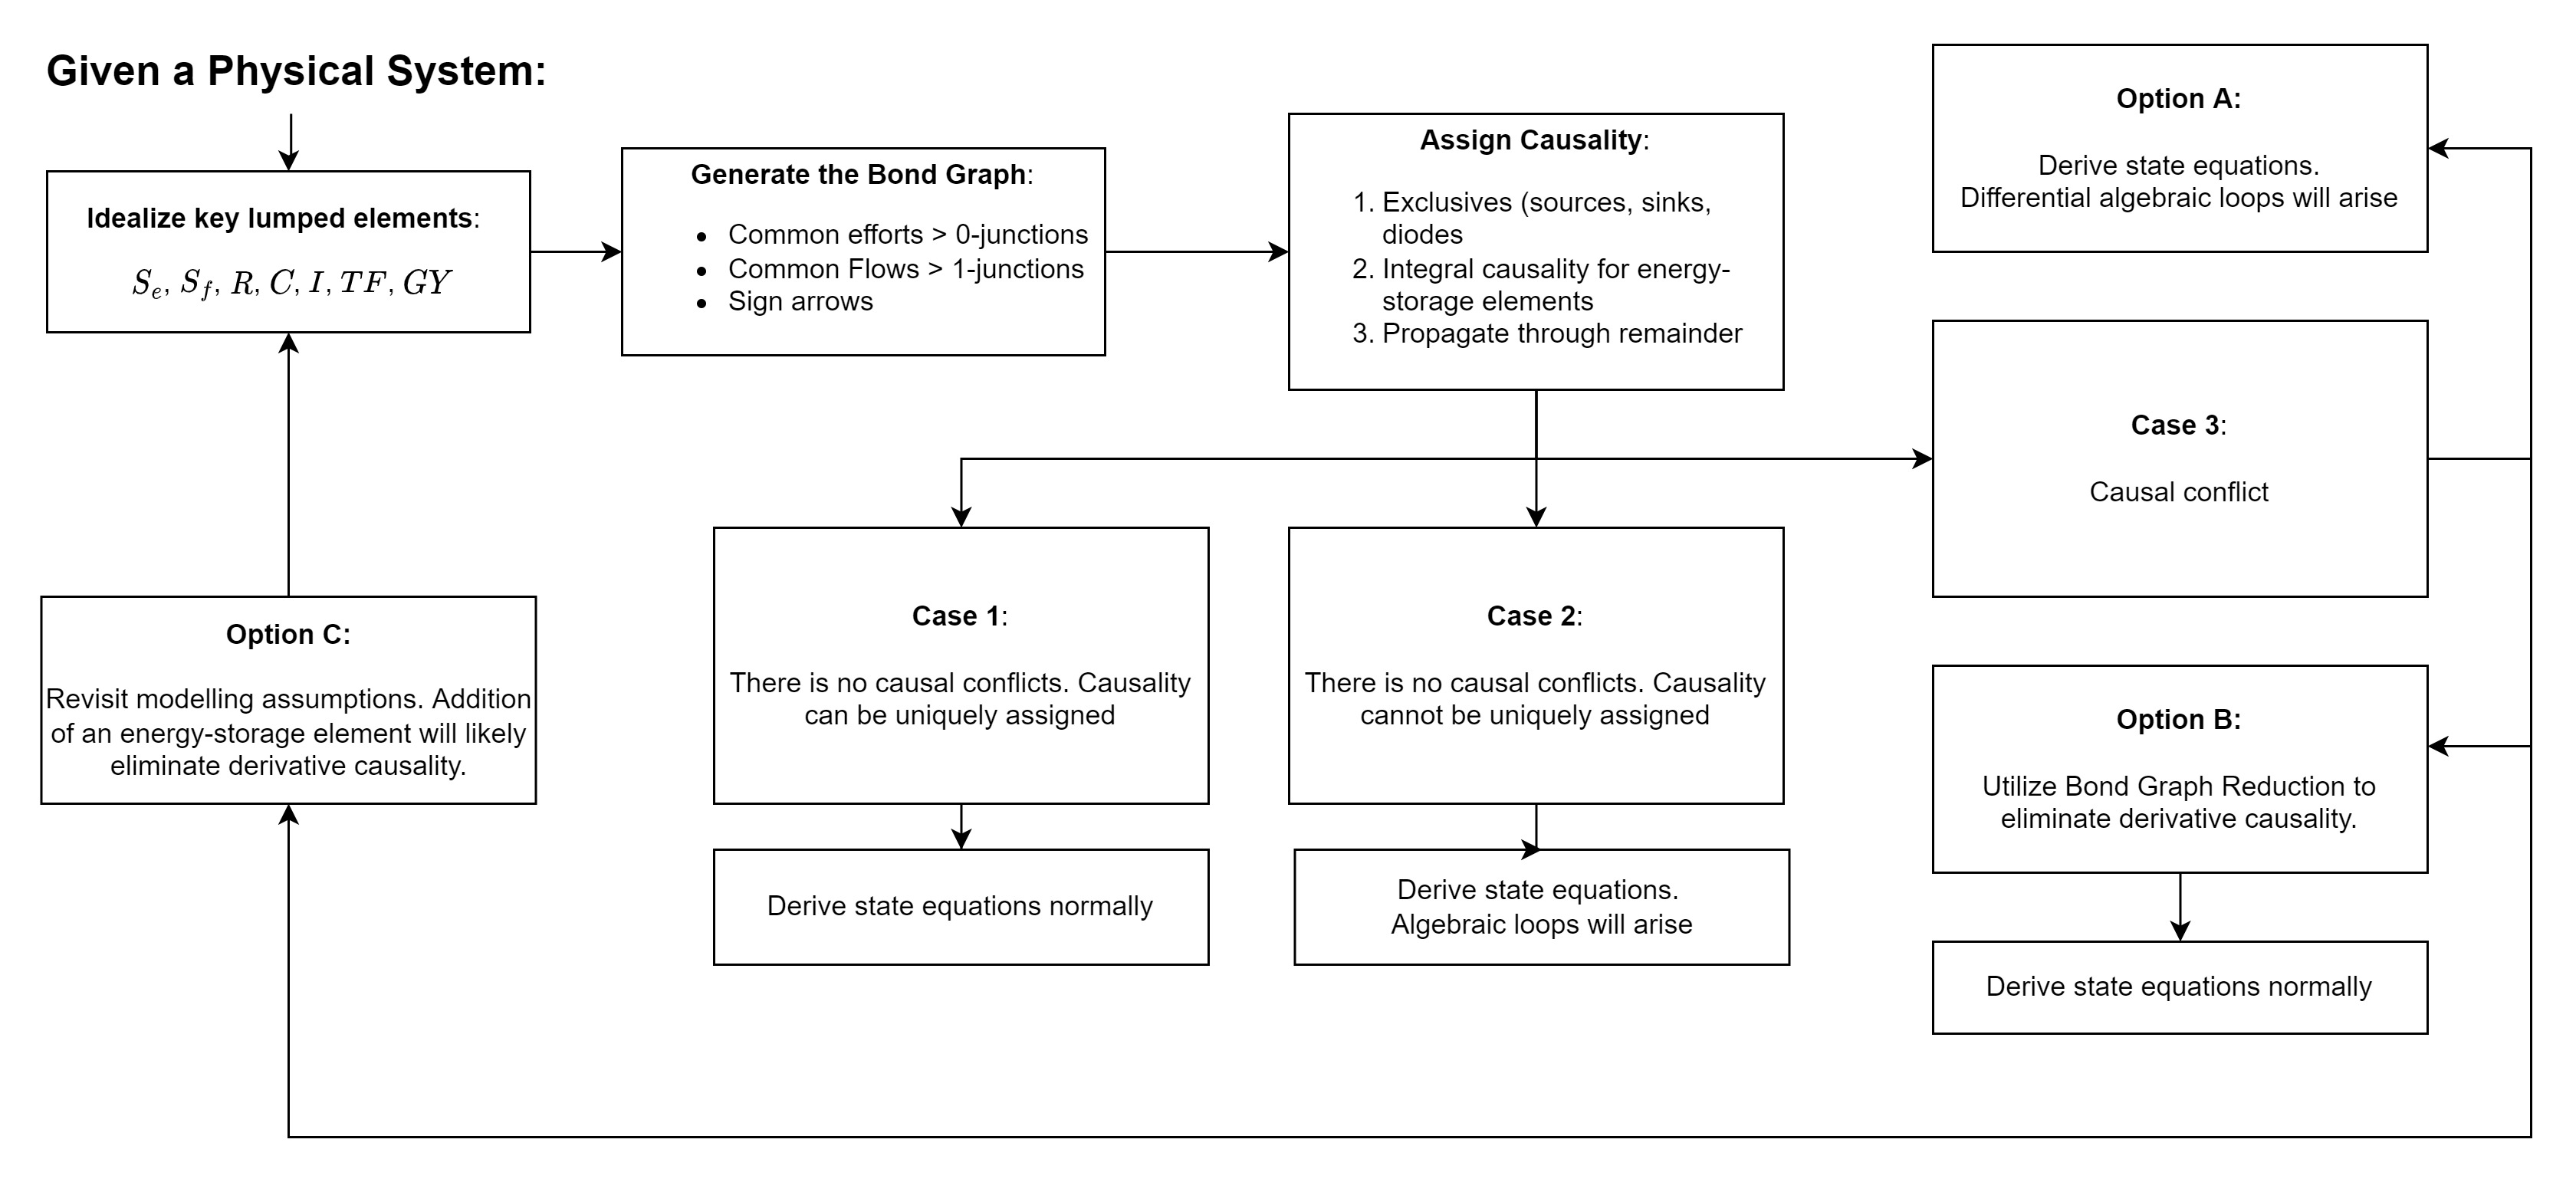
\includegraphics[width=\textwidth]{BondGraphFlowchart.jpg}
\end{figure*}

% \subsection*{Efforts and Flows}
\begin{footnotesize}
\begin{table*}[h]
    \centering
    \begin{tabular}{|l|l c|l c|}
    \hline
         \textbf{Domain}& \textbf{Effort} & & \textbf{Flow}  &\\
         \hline
         Mechanical  & & & &\\
             \tabitem Translational  & Force &\([N]\) & Velocity& \([m/s]\) \\
             \tabitem Rotational    & Torque &\([Nm]\) & Angular Velocity &\([rad/s]\) \\
          \hline
          Electrical & Voltage &\([V]\) & Current &\([A]\)\\
          \hline
          Magnetic & Magnetomotive Force & \([A\cdot\text{turns}]\) & Magnetic Flux Rate &\([Weber/s = V]\) \\
          \hline
          Fluidic &&& &\\
          \tabitem Incompressible & Pressure &\([N/m^2]\) & Volume Flow Rate &\([m^3/s]\) \\
          \tabitem Compressible & Specific Enthalpy &\([Nm/kg]\) & Mass Flow Rate & \([kg/s]\)\\
          \hline
          Thermal & Temperature &\([K]\) & Entropy &\([Nm/Ks]\) \\
          \hline
          Chemical & Chemical Potential & \([J/mol]\) & Molar Flow Rate & \([massflow/Z] ^*\)\\
          \hline
    \end{tabular}
\end{table*}
\end{footnotesize}









\begin{comment}
    % what the option boxes correspond to
    % adds an element, and bond with labels
    \bgComponentWithBondLabel  
    {leave empty}
    {designation}
    {element label}
    {relative to=}
    {other node designation}
    {bond style}
    {leave empty}
    {effort label}
    {flow label}
\end{comment}

\begin{comment}
    % what the option boxes correspond to
    % adds an element, and bond
    \bgComponent{leave empty}
    {designation}
    {element label}
    {relative to=}
    {other node designation}
    {bond style}
\end{comment}

\begin{comment}
    % what the option boxes correspond to
    % adds an element
    \bgComponentNoBond
    {designation}
    {element label}
\end{comment}
\end{document}